\selectlanguage{english}%

\chapter{Controle Fuzzy} \label{capControle}
\epigraph{Se você entende como o universo funciona, de certa forma pode controlá-lo.}{Stephen Hawking}

Neste capítulo, busca-se realizar a sintonia de controladores por realimentação de estados do modelo TS utilizado.

\section{Sistema Aumentado}
 A \jhhref{figModRealim}{Figura} apresenta o sistema em malha fechada.

\begin{figure}[H]
	\begin{centering}
		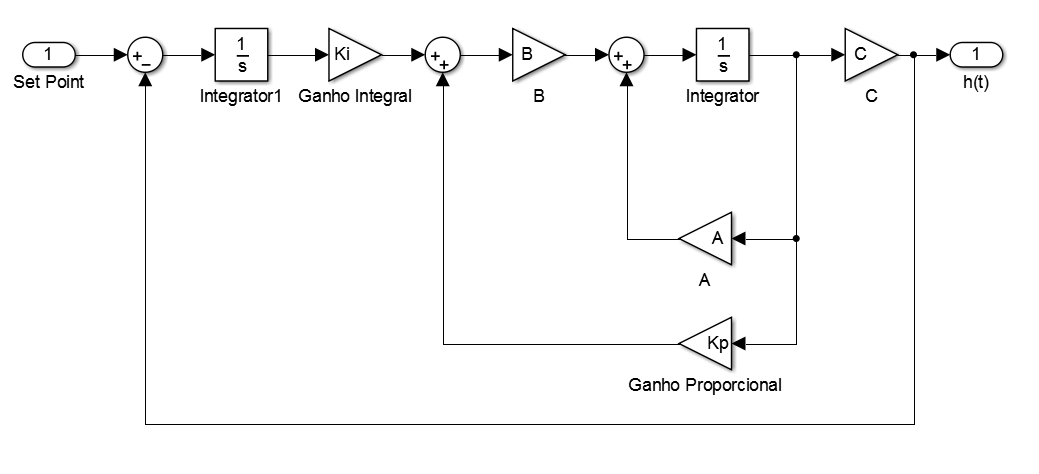
\includegraphics[width=\textwidth]{img/modelo_controlado.png}
		\par\end{centering}
	\caption{\label{figModRealim}Sistema em Malha Fechada}
\end{figure}

O controlador realizado consiste em aplicar um ganho $K = [Kp \ \ Ki]$ sobre o vetor espaço de estados. As condições buscadas são simplesmente erro nulo em regime permanente e estabilidade do sistema. Para a primeira, realiza-se a expansão do espaço de estado, acrescentando as integrais do erro em relação à referência para as duas variáveis controladas (níveis 1 e 2).

\section{Método de Lyapunov}
A utilização de LMIs é uma abordagem prática e eficiente para garantir a estabilidade de sistemas fuzzy. Baseando-se no método de Lyapunov \cite{lyapunov}, desenvolvem-se as LMIs que aplicadas a cada um dos sistemas que compõem o TS final garantem sua estabilidade em malha fechada \cite{mozelli}.

O método direto de Lyapunov é baseado na positividade de funções. Define-se então:

\begin{mydef}
Uma função escalar contínua $w: \mathbb{R}^n \rightarrow \mathbb{R}$, $w(0) = 0$ é semidefinida positiva se, e somente se

	\begin{equation}
		w(x) \geq 0, \forall \ \ x \in \mathbb{R}^n - {0}
	\end{equation}
	Caso desigualdade seja estrita, então $w$ será definida positiva. Uma função \textbf{g} é dita semidefinida (definida) negativa caso \textbf{-g} seja semidifenida (definida) positiva.
\end{mydef}

O método de Lyapunov consiste em encontrar uma função que seja sempre positiva e que decaia à medida que o estado do sistema avance. Sua formalização é dada pelo \jhhref{teoLyapunov}{Teorema} a seguir:

\begin{myteo} \label{teoLyapunov}
	Um sistema dinâmico autônomo é globalmente estável se existe uma função escalar $V : \mathbb{R}^n \rightarrow \mathbb{R} $ tal que:
	
	\begin{itemize}
		\item V é definida positiva
		\item V possui derivada de primeira ordem
		\item $\dot{V}$ é definida negativa
		\item $V \rightarrow \infty$ a medida em que $\|x\| \rightarrow \infty$
	\end{itemize}
\end{myteo}

Assim, uma função V que satisfaça todo os requisitos do Teorema 1 para um dado sistema é chamada de função de Lyapunov. 

\section{Estabilidade De Sistemas}
Para o sistema dinâmico contínuo e invariante no tempo definido pela \jhhref{eqSisSimple}{Equação} a seguir:
\begin{equation} \label{eqSisSimple}
	\dot{x}(t) = Ax(t) + Bu(t)
\end{equation}
Aplicando-se o teorema de Lyapunov \cite{wang}, definindo uma matriz P, chega-se à:

\begin{myteo}
	O equilíbrio de um sistema dinâmico (\ref{eqSisSimple}) é globalmente assintoticamente estável se existe uma matriz P, tal que:
	\begin{align*}
		&P=P'  \\
		&P > 0 \\
		&A'P + P A < 0
	\end{align*}
\end{myteo}

%TODO!!!!
\section{Estabilidade Fuzzy}
Para um modelo TS, simular ao na \jhhref{eqModTakSug}{Equação}, tem-se:
\begin{align*}
	\dot{x}(t) = \frac{\sum_{i=1}^{4}  w_i(c(t))(A_i  x(t) +  B_i  u(t))}{\sum_{j=1}^{4} w_j(c(t))} \vspace{0.5cm}
\end{align*}

Simplificando os termos de ativação de forma a obter um parâmetro A(c), definido como:
\begin{align*}
	\alpha_i (c(t)) &:= \frac{w_i(c(t))}{\sum_{j=1}^{r}w_j(c(t))} \\
	A(\alpha) &:= \sum_{i=1}^{r} \alpha_i (c(t))A_i
\end{align*}

Aplicando-se a Teoria de Lyapunov, como proposto por Tanaka e Wang \cite{wang}, uma vez que o modelo final é convexo, basta tratar a \jhhref{eqLyapXk}{Equação} nos vértices do sistema, ou seja, em cada um dos sistemas que compõem as \jhhref{eqRegraIGeral}{Regras}. 
A análise computacional via LMIs possibilita a busca por uma matriz P que satisfaça essas condições, caso ela exista, prova-se a estabilidade do sistema. Assim, o sistema TS é globalmente assintoticamente estável \cite{tanakaWang} existe solução para:

\begin{align} \label{eqLyapXk}
	encontre \ \ &P \nonumber \\
	s.a \ \ &P \succ 0 \nonumber \\
	&A_i'P + P A_i \prec 0, \ \ i=1,2,3, ... , r
\end{align}

Seguindo estas premissas \cite{wang}, obtém-se o seguinte teorema:
\begin{myteo} \label{teoControlador}
Dado um sistema fuzzy Takagi-Sugeno, convexo, composto por r regras e modelos correspondentes, em malha fechada com ganhos $K_i = M_i X^{-1}$, sua estabilidade é verificada se existe solução para o problema
	\begin{align} \label{eqContFuzzy}
		encontre \ \ &X = X', \ \ i = 1,2,...,r \nonumber \\
		&X \succ 0 \nonumber \\
		s.a \ \ & 
		\begin{bmatrix}
			X	&	XA_i' - M_i'B_i'  \\
			A_iX - B_iM_i &	X
		\end{bmatrix} \succ 0 \nonumber \\
	\end{align}
\end{myteo}

\selectlanguage{brazil}%

